

Apache Storm is a distributed analytics framework that acts as a transformation pipeline on data streams. The basic components of the Storm pipeline are data emitters (Spouts), data transformers (Bolts), and data streams (tuples). These components are organized into Topologies, which define the workflow as a directed acyclic graph of Spouts and Bolts connected by tuple streams. Streams and Bolts run in one or more JVM managed by Workers which are in turn provisioned by Supervisors. To deploy a topology, the serialized code and configuration are sent to a master node (Nimbus) which calculates a deployment strategy and delegates work to the Supervisor through Zookeeper.



\subsubsection{Storm Overview}

\begin{figure}[H]
\centering
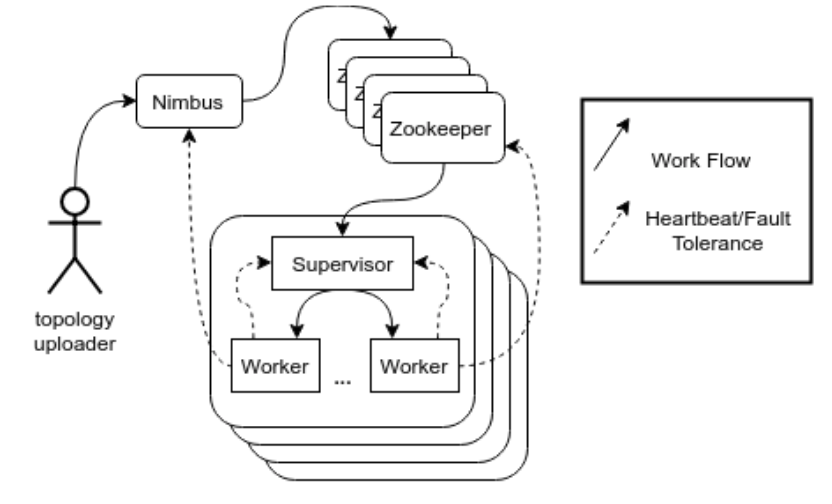
\includegraphics[scale=.4]{img/storm_cellar/storm_arch.png}
\caption{Storm Architecture}
\label{fig:storm_arch}
\end{figure} 

\textbf{Work flow}
\begin{enumerate}
\item Topology submitter uploads topologies to Nimbus. Information uploaded includes topology.jar, serialized topology code, serialized topology configuration. 
\item Nimbus calculates assignments - looks at topology configuration, parallelism definitions, relationships between spouts and bolts. Figures out how to assign work and pushes that to zookeeper.
\item Supervisor nodes receive assignments through watches/sets in zookeeper. 
\item Supervisor nodes download topology.jar, serialized topology configuration from nimbus
\item Supervisor spawns worker JVM processes to execute topology
\end{enumerate}



\textbf{Fault tolerance}
\begin{itemize}
\item Workers heartbeat back to supervisors and nimbus via zookeeper and locally(for redundancy if zookeeper goes down)
\item If worker goes down the supervisor auto restarts it. if it dies repeatedly nimbus picks up on that and blacklists that supervisor, redistributing work to other sup nodes
\item If nimbus goes down, deployed topos still work but new ones cant be uploaded
\item Keeping connections generic to not confuse different control and data flow functionality. Different speaker pairs for worker internal comms, authentication (kerberos, http basic, filesystem, user, ZK, dashboard, ...)
\end{itemize}





\subsubsection{Implementation}

\begin{figure}[H]
\centering
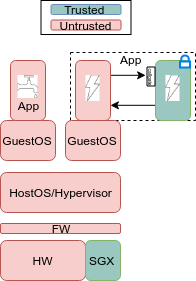
\includegraphics[scale=.7]{img/storm_cellar/sgx_threat_model_003.png}
\caption{Threat Model}
\label{fig:threat_model_003}
\end{figure}

Our threat model uses the standard assumptions inherited from SGX. Namely, 
\begin{itemize}
\item We trust Intel, the implementation of SGX, and the CPU package which contains it. 
\item We trust the application developed (Storm in this case) is hardened and vulnerability free (no SQLi or BoF). Enclaves don't protect against bad code. 
\item We don't consider DoS or side channels for this research (@TODO?), although SGX-LKL\cite{Priebe_Muthukumaran_Lind_Zhu_Cui_Sartakov_Pietzuch_2019, Zheng_Dave_Beekman_Popa_Gonzalez_Stoica_2017} does implement oblivious call interface to mitigate access pattern analysis.
\item The attacker is located locally on the OS or hypervisor and has full control over the host running the application.
\end{itemize}


The approach identified below protects for aggregated output from workers (spouts and bolts). If sources and topologies need shielded as well we could run the nimbus master in an enclave and terminate Talos\cite{Aublin_Kelbert_OKeeffe_Muthukumaran_Priebe_Lind_Krahn_Fetzer_Eyers_Pietzuch_2017} TLS connections in enclaves as well. 

While Nimbus, Zookeeper, and Supervisors may contain sensitive information about the architecture of the topology (and more...), the components that operate on data directly are Spouts and Bolts. This work focuses on partitioning storm to provide confidentiality and integrity guarantees over the data stream pipeline, and leaves control and management plane security for future work.



\begin{figure}[h]
\begin{tabular}{p{0.48\textwidth}p{0.47\textwidth}}
\begin{minipage}{.48\textwidth}
\centering
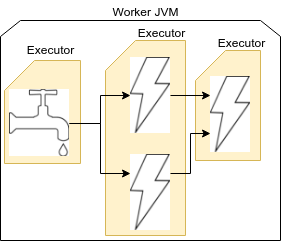
\includegraphics[scale=.4]{img/storm_cellar/storm_topo_single_jvm.png}
\subcaption{Single JVM}
\label{fig:storm_topo_single}
%\end{figure} 
\end{minipage}
&
\begin{minipage}{.47\textwidth}
\centering
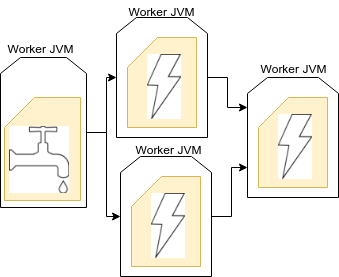
\includegraphics[scale=.4]{img/storm_cellar/storm_topo_multi_jvm.png}
\subcaption{Multi-JVM}
\label{fig:storm_topo_multi}
\end{minipage}
\end{tabular}
\caption{Parallelism in Storm }
\end{figure}

\subsubsection{Parallelism}

Storm’s distributed processing pipeline creates a natural boundary for partitioning data stream constructs in enclave execution. Parallelism in the Storm data plane comes in 2 flavors - thread and process. 

\textbf{Thread parallelism }dictates the number and types of Executors inside a worker JVM.

\textbf{Process parallelism} dictates the number of Worker JVM nodes across the cluster.

\textbf{Inter-process} communication uses network I/O to pass tuple streams between Worker nodes (Netty). Each Worker node runs a listener thread that puts incoming tuples on a message queue for processing. To prevent eavesdropping or data modification, it’s necessary to terminate this connection along with the receive queue inside an enclave. Within the Worker process, a second queue is used to feed data to the Spout/Bolt threads for processing. Again, it is necessary to place both the data transfer queues and the processing logic inside an enclave. The result is pictured in Figure \ref{fig:storm_part} where the shaded region is run in an enclave. 

 \textbf{Inter-thread} messaging occurs within the same JVM and is implemented with LMAX disruptor queues. Each thread has high performance, non-blocking ring buffer. Inter-thread messaging can use symmetric encryption on LMAX so we need to test performance of both (assumed in Figure \ref{fig:storm_part}). We are not considering anchoring/message guarantees in initial tests due to overhead.
 
To scale distributed computation, increase the number workers for topology and increase the number of tasks run in parallel.Each worker runs multiple threads called executors. Executors run one or more tasks (spouts or bolts).

\begin{figure}[H]
\centering
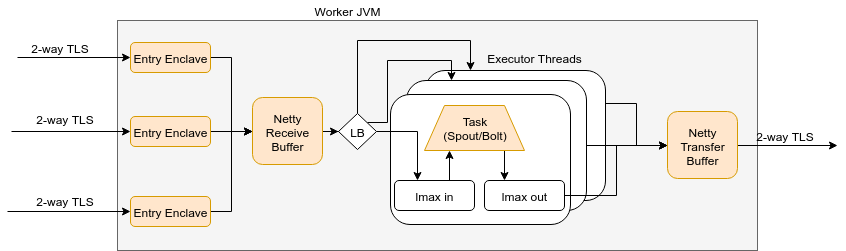
\includegraphics[scale=.5]{img/storm_cellar/storm_part.png}
\caption{Storm Enclave Partitioning}
\label{fig:storm_part}
\end{figure}

The resulting Worker process, depicted in Figure \ref{fig:storm_part} with enclave components shaded, forms the basic building block for SGX-enabled Storm topologies. Tuple streams arrive at a Worker from the network and are stored in a network I/O optimized receive buffer (Netty queue).  Within the Worker process, tuples are read from the Netty receive queue into a thread-safe ring buffer(LMAX Disruptor) which routes tuples to Spout/Bolt threads for processing. Spouts and Bolts then put results onto the outgoing Disruptor queue which in turn feeds into the outgoing Netty queue for transfer over the network to the next Worker in the processing pipeline. 

Our build process uses the publicly available source repositories for SGX-LKL and Netty. We setup resources using Vagrant to simplify testing and rebuilding on local or remote hosts. We have developed a set of custom Ansible roles and plays to make this work as modular and reusable as possible. Only a slight modification to the Apache Storm source to inform the Supervisor to spawn Workers inside an enclave. As described in Section \ref{sec_sgx}, \textit{fork()} syscall is prohibited from within an enclave, so it is necessary to EEXIT before launching the Worker JVM. 